\chapter{Изучение реакции перезарядки
  \maybebm{{\dpchex}}}
В последнее время возобновился интерес к извлечению  информации о сечениях
спин-зависящей части $np$-рассеяния из реакций перезарядки на дейтроне.
Заинтересованность в подобных исследованиях была связана, в частности, с
ускорением дейтронов с энергией выше 1~ГэВ на нуклон на ускорительном комплексе
ЛФВЭ ОИЯИ.

Данная глава посвящена изучению зарядово-обменных процессов в дейтрон-протонных
соударениях полученных с помощью водородной пузырьковой камеры. Мотивацией этих
исследований явилось отсутствие, к началу наших исследований, информации о
спин-зависящей амплитуде \np рассеяния, измеряемой в реакции перезарядки
неполяризованного дейтрона на неполяризованном протоне-мишени при энергиях 1~ГэВ
и выше. Целями исследований было:

\begin{itemize}
\item Получить значение дифференциального сечения реакции перезарядки \dpchex
  при нулевой передаче четырёхимпульса на основе материала с водородной
  пузырьковой камеры.
\item Подготовить электронный эксперимент (установка СТРЕЛА) для измерений
  дифференциального сечения реакции перезарядки на дейтроне.
\end{itemize}

Прежде чем перейти к более детальному описанию результатов эксперимента кратко
опишем материал, на основе которого была проведена оценка вклада спин-зависящей
части амплитуды элементарного \np рассеяния и предложен (следующая глава)
электронный эксперимент на установке СТРЕЛА.

\section{Методика эксперимента}
Экспериментальный материал был получен с помощью 100-см водородной пузырьковой
камеры на синхрофазотроне ЛВЭ ОИЯИ~\cite{belon65}, экспонированной пучком ядер
дейтерия. Материал содержит два набора данных, полученных в неполяризованном и
поляризованном пучке дейтронов.

Жидководородная пузырьковая камера является одновременно чистой протонной
мишенью и детектором, регистрирующим почти все испущенные из точки
взаимодействия вторичные заряженные частицы, траектории которых
восстанавливались в условиях 4$\pi$-геометрии. Камера была помещена в сильное
магнитное поле (средняя величина напряжённости равна
$\sim 1.85$~T)~\cite{glagolev94}. Это позволило надёжно идентифицировать
вторичные заряженные частицы по знаку заряда и с высокой точностью определять их
импульсы с помощью измерения кривизны треков, а для останавливающихся частиц
восстанавливать импульс по пробегу. Величины зарядов оценивались по
ионизационным потерям.

Камера была облучена выведенным из синхрофазотрона пучком дейтронов с импульсом
3.35~ГэВ/с~\cite{glagolev72}. Использование ядерных пучков, падающих на
неподвижную протонную мишень приводит к тому, что все фрагменты ядра являются
быстрыми в лабораторной системе координат, и таким образом они могут быть
надёжно зарегистрированы. При этом заряженные фрагменты могут быть хорошо
измерены и идентифицированы практически без потерь. Эти условия позволяли
изучать реакции, содержавшие не более чем одну нейтральную частицу в
эксклюзивном подходе. Таким образом, преимущества изучения дейтрон-протонных
взаимодействий (так называемая обратная геометрия) являются очевидными в отличие
от протон-дейтронных взаимодействий. Восстанавливалась практически без потерь
полная кинематика событий.

Детальное описание экспериментальной установки и системы обработки может быть
найдено в работах~\cite{belon65,alad75,alad73}. Автором диссертации для решения
поставленной задачи~--- изучение зарядово-обменных процессов в дейтрон-протонных
соударениях, была использована уже сформированная лента суммарных результатов
(DST), на которой число событий реакции \dpfrag превысило 10$^{\,5}$.

\subsection{Обработка снимков}
Снимки, полученные в течение ряда экспозиций пузырьковой камеры, обрабатывались
по стандартной схеме: двухкратный просмотр стереофотографий с регистрацией
наблюдаемых событий, измерение координат точек на треках в плоскости плёнок и
визуальная оценка плотности следов (ионизации) заряженных вторичных частиц.
Далее проводилась математическая обработка на ЭВМ результатов измерений,
включающая в себя восстановление пространственной картины взаимодействий и отбор
физических гипотез с помощью программ кинематической идентификации.

Измерения на трёх проекциях использовались для геометрической реконструкции и
последующего кинематического анализа событий. Если событие было отбраковано на
любом этапе обработки, все проекции повторно измерялись. Для реконструкции
событий использовались адаптированные версии библиотеки программ
пространственной реконструкции и кинематического анализа событий
CERN HYDRA~\cite{framer82}.

Результаты измерения отобранных событий, вместе с набором входных параметров,
характеризующих топологию магнитного поля в камере и оптическую систему,
использовались для геометрического восстановления событий. В процессе
геометрической реконструкции события вычислялись радиус кривизны ($r$),
азимутальный ($\varphi$) и полярный ($\lambda$) углы для всех заряженных частиц,
принадлежащих одной вершине, а также матрица ошибок.

Для работы программы кинематического анализа был введён блок гипотез, который
содержал список комбинаций всех возможных вторичных заряженных частиц в
событиях. Второй блок содержал значения импульса, угла наклона и азимутального
угла вместе с их ошибками для пучковых частиц во входной плоскости камеры.
Кинематический анализ проводился для гипотез 4С-FIT (в конечном состоянии только
заряженные частицы) и 1С-FIT (в конечном состоянии только одна нейтральная
частица). По недостающей массе и критерию $\chi^2$ оценивалась достоверность
возможных гипотез, а также уточнялись значения кинематических параметров
(импульс и энергия) частиц. События, которые не удовлетворяют FIT-гипотезам, но
значение недостающей массы такое, что она не противоречит гипотезе с
образованием двух или более нейтральных частиц, относились к группе
нефитированных (NOFIT-гипотезы).

Последним этапом в обработке снимков с водородной камеры являлась идентификация
каналов взаимодействия, которая производилась по значению $\chi^{2}$ и
сопоставлением ионизационных потерь, вычисленных программой GEOKIN с визуальной
оценкой. Для кинематических гипотез, удовлетворяющих критериям идентификации,
формировалась лента суммарных результатов.

Детальное описание процесса обработки, кинематического анализа, критериев отбора
гипотез и формирования DST приведено в ряде работ, выполненных с помощью 100-см
водородной пузырьковой камеры~\cite{glagolev76,kachara88,niora91}.

\section{Анализ реакции \maybebm{{\dpfrag}}}
Полученный экспериментальный материал, записанный после обработки на ленту
суммарных результатов, содержит 237413 событий $dp$-взаимодействия. Информация о
всех наблюдавшихся 17 каналах реакции $dp \rightarrow X$ представлена в
таблице~\ref{tab:dp_channels}.
\begin{table}[!h]
  \begin{center}
    \bigskip
    \resizebox{0.35\textheight}{!} {
      \begin{tabular}{|r|l|c|}
        \hline \No & Реакция & Число событий \\ \hline \hline
        1  & $dp \rightarrow ppn$ & 102778 \\ \hline
        2  & $dp \rightarrow p\pi^{+}nn$ & 65284 \\ \hline
        3  & $dp \rightarrow ppn\pi^{0}$ & 31295 \\ \hline
        4  & $dp \rightarrow dp$ & 16184 \\ \hline
        5  & $dp \rightarrow ppp\pi^{-}$ & 5487 \\ \hline
        6  & $dp \rightarrow d\pi^{+}n$ & 4963 \\ \hline
        7  & $dp \rightarrow dp\pi^{0}$ & 3950 \\ \hline
        8  & $dp \rightarrow d\pi^{+}n\pi^{0}$ & 1843 \\ \hline
        9  & $dp \rightarrow dp\pi^{0}\pi^{0}$ & 1839 \\ \hline
        10 & $dp \rightarrow dp\pi^{+}\pi^{-}\pi^{0}\pi^{0}$ & 1414 \\ \hline
        11 & $dp \rightarrow pp\pi^{+}\pi^{-}n$ & 1163 \\ \hline
        12 & $dp \rightarrow dp\pi^{+}\pi^{-}$ & 576 \\ \hline
        13 & $dp \rightarrow \pi^{+}\pi^{+}nnn$ & 315 \\ \hline
        14 & $dp \rightarrow ppp\pi^{-}\pi^{0}$ & 167 \\ \hline
        15 & $dp \rightarrow ppp\pi^{-}\pi^{0}\pi^{0}$ & 67 \\ \hline
        16 & $dp \rightarrow pp\pi^{+}\pi^{-}n\pi^{0}$ & 49 \\ \hline
        17 & $dp \rightarrow dp\pi^{+}\pi^{-}\pi^{0}$ & 39 \\ \hline
        \hline $\sum$ & $dp \rightarrow X$ & 237413 \\ \hline
      \end{tabular}
    }
    \bigskip
    \caption{Перечень всех наблюдавшихся каналов реакций в дейтрон-протонных
      столкновениях, полученных с помощью 100-см водородной пузырьковой камеры.}
    \label{tab:dp_channels}
  \end{center}
\end{table}



%%% Local Variables:
%%% mode: latex
%%% TeX-master: "../musinsky_disser"
%%% coding: utf-8
%%% End:


В диссертации подробно изучалась кинематически полностью восстанавливаемая
реакция \dpfrag. Методика выделения и идентификации реакции развала дейтрона
\dpfrag от конкурирующих каналов подробно рассмотрена в
работах~\cite{alad75,alad73}.

Из таблицы~\ref{tab:dp_channels} видно, что приблизительно половина всех событий
дейтрон-протонных соударений, составляла реакция безмезонного развала дейтрона
\dpfrag. Эта реакция может идти как:

\begin{itemize}
\item \dpchex~--- реакция перезарядки с изменением зарядового состояния
  протона-мишени, или
\item \dpret~--- реакция прямого канала с сохранением заряда протона-мишени.
\end{itemize}
В дальнейшем класс событий изучаемой реакции будем называть перезарядкой, если в
системе покоя налетающего дейтрона среди вторичных продуктов самой быстрой
частицей является нейтрон. Другой класс событий, где такой частицей является
один из двух протонов, относится к прямому каналу с сохранением заряда
протона-мишени. После применения такого разделения получаем 17512 событий
реакции перезарядки и 85266 событий прямого канала.

Как хорошо разделяются эти два класса событий можно видеть на
рис.~\ref{fig:chex_ret_t}, где приводятся их распределения по величине квадрата
переданного четырёхмерного импульса $|t|$ для реакции перезарядки
(заштрихованное) и реакции прямого канала (незаштрихованное). Инвариантная
величина $|t|$ экспериментально определяется как квадрат четырёхмерного
переданного импульса от протона-мишени к нейтрону в лабораторной система
координат. Такое определение $t$ не зависит от того, какой из протонов является
продуктом взаимодействия.

\begin{figure}[h]
  \centering
  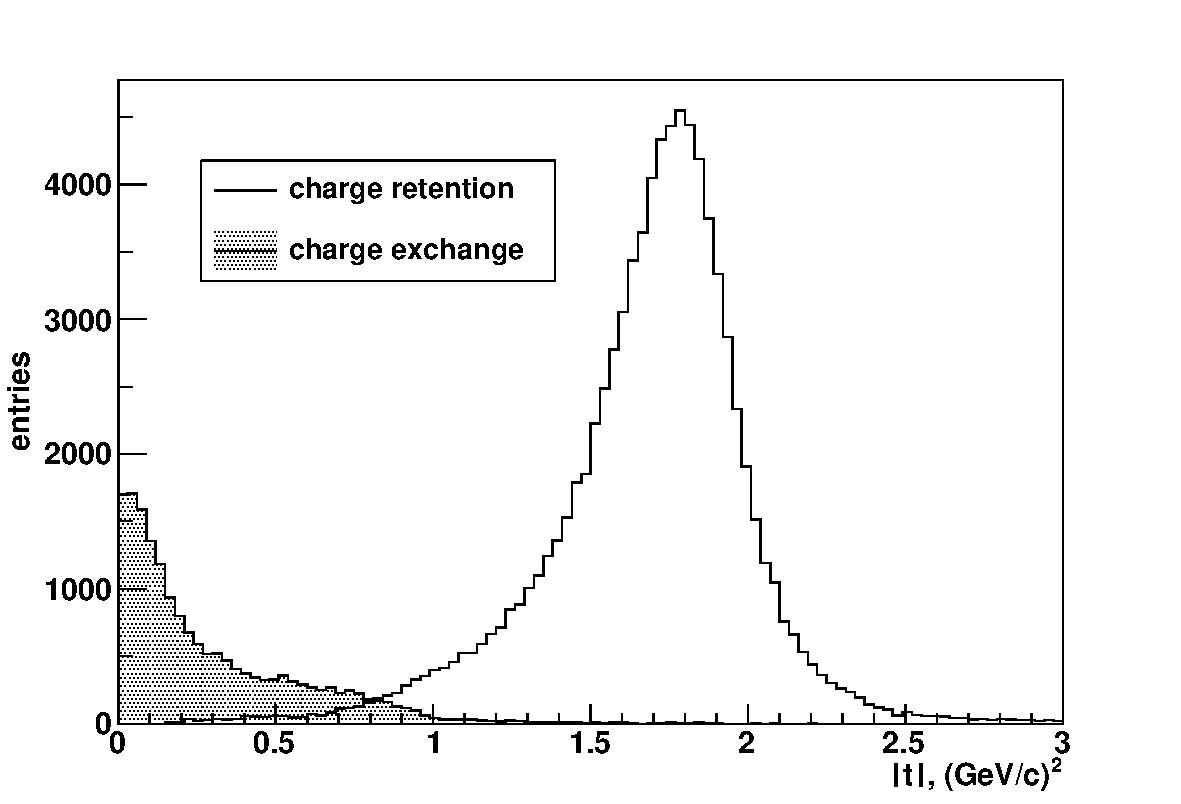
\includegraphics[width=1.00\textwidth]{chex_ret_t.pdf}
  \caption{Распределения событий реакции \dpfrag по квадрату четырёхмерного
    переданного импульса $|t|$ от протона-мишени к нейтрону. Заштрихованное
    распределение (charge exchange)~--- канал реакции перезарядки \dpchex,
    незаштрихованное (charge retention)~--- прямой канал реакции развала
    дейтрона \dpret.}
  \label{fig:chex_ret_t}
\end{figure}

В случае реакции перезарядки на дейтроне, благодаря применяемой методике
исследования (пучок ускоренных дейтронов), в конечном состоянии в лабораторной
системе координат наблюдается характерная топология событий~--- два выходящих
из точки взаимодействия быстрых протона с близкими импульсами и малым углом
раствора. Это способствует надёжному разделению на стереофотографиях реакции
перезарядки \dpchex с реакцией прямого канала развала дейтрона \dpret, в которой
один из двух протонов всегда медленный, что позволяет исследовать реакцию
перезарядки практически без потерь~\cite{balga88}.

Экспериментальные данные о реакции \dpfrag свидетельствуют о том, что этот
процесс, в основном, идёт с участием одного нуклона из дейтрона, тогда как
другой нуклон является спектатором. Спектатор~--- самый медленный из нуклонов в
системе покоя дейтрона (антилабораторная система), не принимавший участие во
взаимодействии (квази-упругое рассеяние). Рассеянным нуклоном называем,
наоборот, самый быстрый из нуклонов в системе покоя дейтрона. Оставшийся
фрагмент~--- нуклон отдачи. На рис.~\ref{fig:spec_reco_scat} приведены
импульсные распределения всех продуктов из реакции безмезонного развала дейтрона
\dpfrag в системе покоя дейтрона.

\begin{figure}[h]
  \centering
  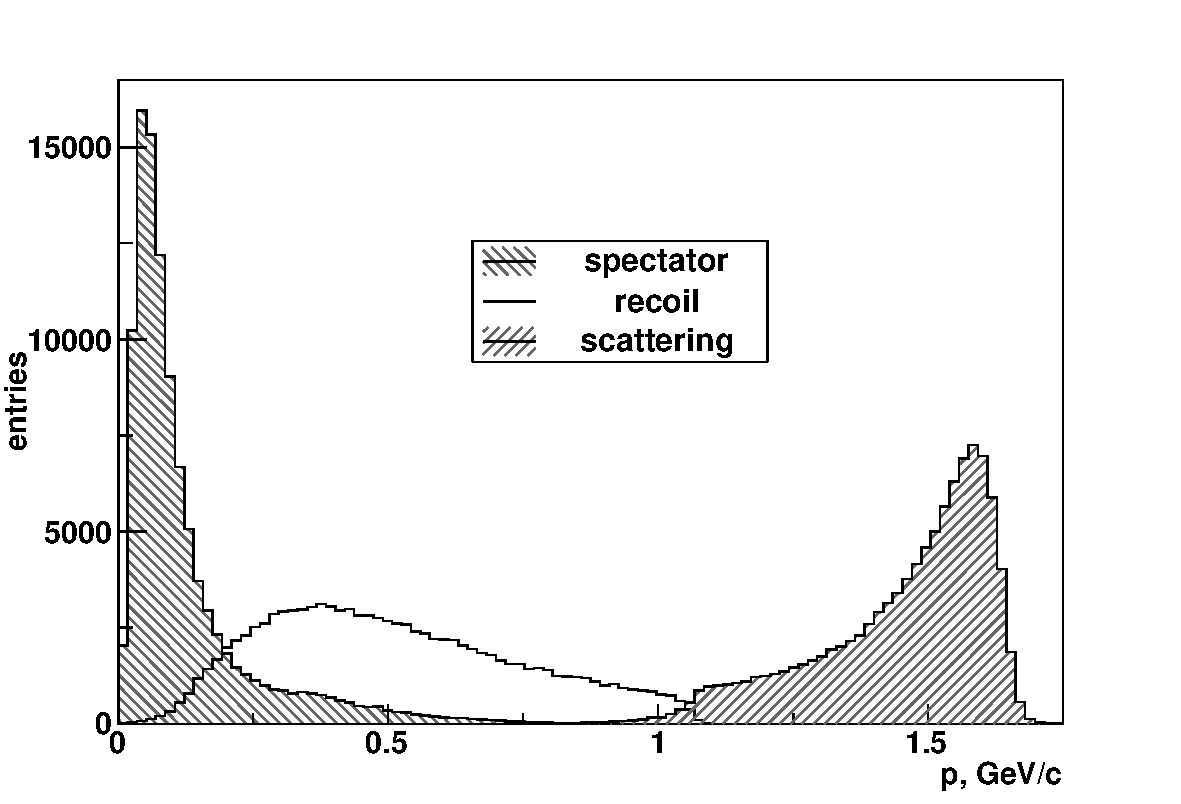
\includegraphics[width=1.00\textwidth]{spec_reco_scat.pdf}
  \caption{Импульсные распределения спектаторов (spectator), нуклонов отдачи
    (recoil) и рассеивающихся нуклонов (scattering) из реакции развала дейтрона
    \dpfrag в системе покоя дейтрона.}
  \label{fig:spec_reco_scat}
\end{figure}

В системе покоя дейтрона и в лабораторной системе координат определения нуклона
отдачи и рассеянного нуклона взаимно изменяются, а именно, нуклон отдачи в
системе покоя дейтрона, тот же, что и рассеянный нуклон в лабораторной системе
координат. В дальнейшем мы будем, как правило, использовать эти обозначения для
системы покоя дейтрона.

Так как при развале быстрого дейтрона \dpfrag в лабораторной системе спектаторы
имеют достаточно большие импульсы и их можно надёжно идентифицировать, потери
обусловлены, главным образом, событиями с малыми передачами импульса
протону-мишени (протону-отдачи). Однако, такие потери меньше, чем при упругом
рассеянии \dpela, так как при развале налетающего дейтрона наблюдается резкое
(примерно в два раза) изменение импульса, а следовательно, и кривизны трека в
магнитном поле у заряженных фрагментов по сравнению с падающим ядром. Кроме
того, для развала дейтрона необходимо затратить энергию порядка 2.2~МэВ (энергия
связи дейтрона), что приводит к отсутствию частиц отдач с малыми импульсами.

\begin{figure}[h]
  \centering
  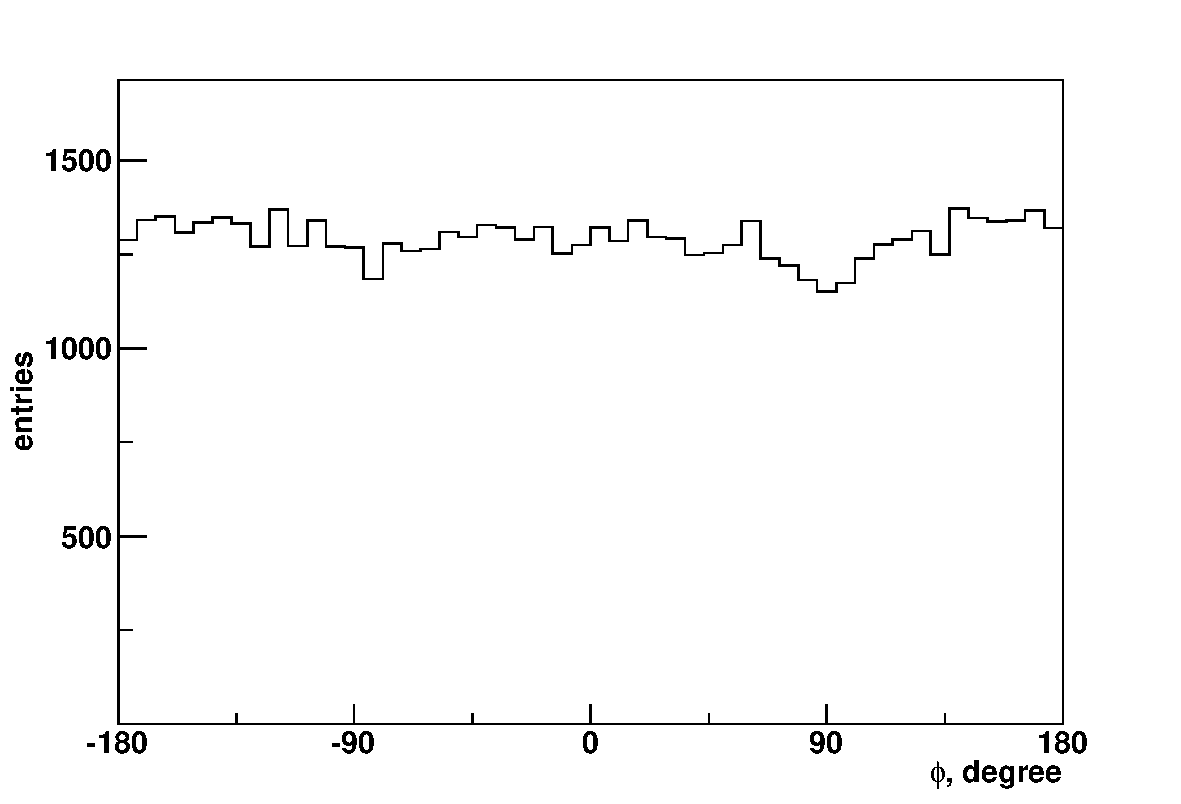
\includegraphics[width=1.00\textwidth]{phi_recoil.pdf}
  \caption{Распределение по азимутальному углу $\phi$ протонов отдачи в реакции
    развала ядра дейтрона \dpfrag.}
  \label{fig:phi_recoil}
\end{figure}

Поскольку надёжное наблюдение треков протонов в водородной камере начинается с
импульса выше приблизительно 80~МэВ/c (что соответствует длине трека в
пузырьковой камере порядка 1~мм)~\cite{niora91}, то потери в отборе событий с
развалом ядра дейтрона можно считать несущественными. Об этом можно судить из
распределения по азимутальному углу протонов отдачи в изучаемом нами канале
развала ядра дейтрона \dpfrag, и также, из распределения по поперечным импульсам
рассеивающихся нуклонов~\cite{alad75_3}. На рис.~\ref{fig:phi_recoil} показано
азимутальное распределение протонов отдачи в реакции развала дейтрона. Видно,
что оно практически изотропно во всём интервале азимутальных углов, т.е. потери
в реакции полного развала ядра дейтрона минимальные, несущественные.

\subsection{Сечение и миллибарн-эквивалент события}
Экспериментальный материал по дейтрон-протонным столкновениям содержит два
набора данных. Первый из них~--- $dp$-взаимодействия, полученные с
неполяризованным пучком в начале 70-х годов, и второй~--- данные, накопленные в
конце 80-х годов в пучке поляризованных дейтронов. Анализ и сравнение некоторых
основных характеристик взаимодействий поляризованных и неполяризованных
дейтронов с протонами показал их идентичность, что позволило объединить оба
набора экспериментальных данных~\cite{balga88}. В работе используются суммарные
данные из обеих наборов.

Для определения миллибарн-эквивалента события, из известного полного сечения
$dp$-реакции, необходимо было оценить экспериментальные потери событий в
$dp$-взаимодействиях. Как уже отмечалось, потери в отборе событий с развалом
ядра дейтрона можно считать несущественными. Основным видом потерь при поиске
событий были потери при малых переданных импульсах в упругих взаимодействиях
\dpela. Это хорошо видно из рис.~\ref{fig:phi_elastic}, где приводятся
распределения по азимутальному углу протонов отдачи в упругом $dp$-канале для
разных интервалов значения $|t|$. Распределения нормированы на максимум, чтобы
лучше показать их различие. Как видно, при малых передачах
$|t| < 0.06$~(ГэВ/с)$^2$ (заштрихованное распределение) наблюдается отклонение
от изотропии, обусловленное потерями в этой области переданного четырёхимпульса.
При более высоких передачах $|t| > 0.06$~(ГэВ/с)$^2$ распределение
(незаштрихованное) становится изотропным.

\vspace{-0.1cm}
\begin{figure}[h]
  \centering
  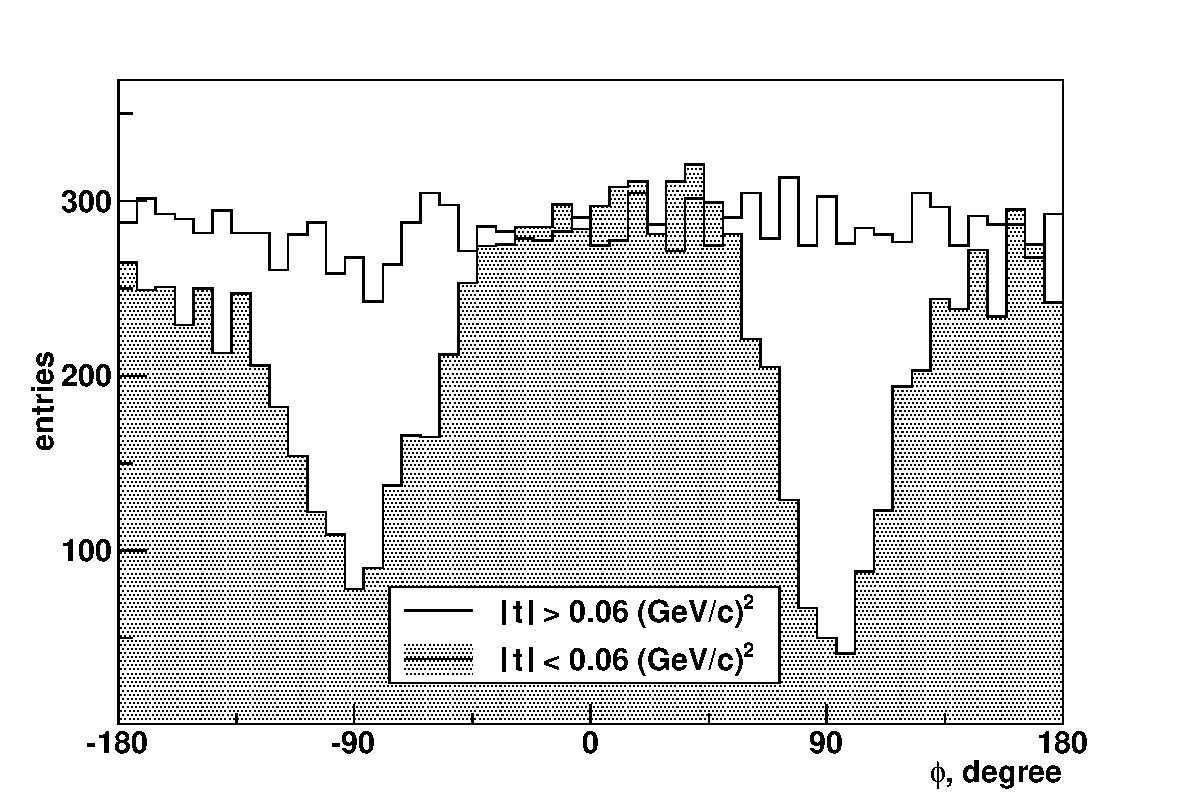
\includegraphics[width=1.00\textwidth]{phi_elastic.pdf}
  \caption{Распределения по азимутальному углу $\phi$ протонов отдачи в реакции
    упругого рассеяния \dpela (нормированы на максимум). Заштрихованное
    распределение при значениях $|t| < 0.06$ (ГэВ/с)$^2$, незаштрихованное при
    $|t| > 0.06$ (ГэВ/с)$^2$.}
  \label{fig:phi_elastic}
\end{figure}

Реально принималось, что случайные потери по каналам реакции $dp \rightarrow X$
пропорциональны вкладам каналов, а систематические потери сосредоточены только в
упругом канале \dpela и связаны с рассеянием на малые углы. Эти потери прямо
отражались на поведении дифференциального сечения упругого $dp$-рассеяния и
оценивались по экспериментальным данным.

\begin{figure}[h]
  \centering
  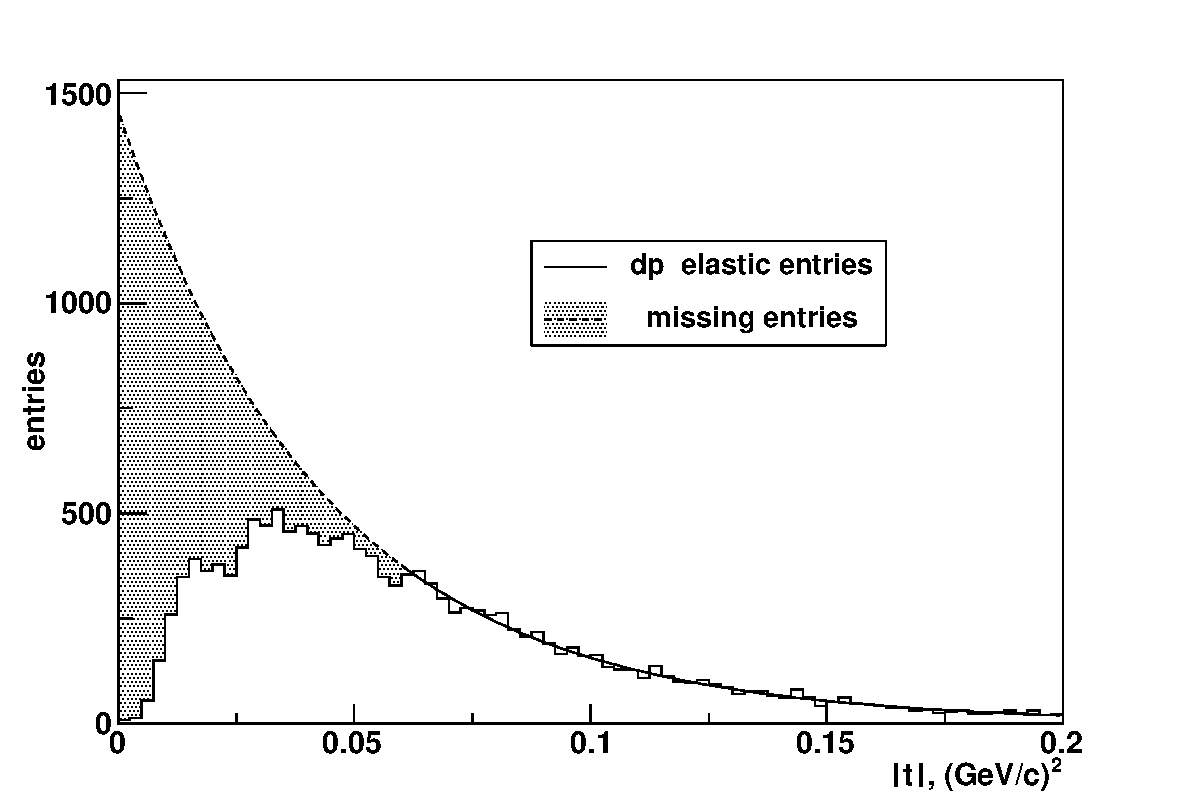
\includegraphics[width=1.00\textwidth]{dp_dp_t.pdf}
  \caption{Распределение событий упругого рассеяния \dpela по квадрату
    четырёхмерного переданного импульса $|t|$. Заштрихованная область (missing
    entries) представляет события потерянные в этом канале. Штриховая линия~---
    экстраполяция аппроксимирующей функцией в область потерь
    $|t| < 0.06$~(ГэВ/с)$^2$.}
  \label{fig:dp_dp_t}
\end{figure}

Число потерянных событий при малых передачах $|t|$ в реакции упругого
$dp$-рассеяния оценивалось путём аппроксимации распределения на
рис.~\ref{fig:dp_dp_t} двойной экспоненциальной функцией и затем экстраполяцией
в область $|t| < 0.06$ (ГэВ/с)$^2$. Процедура аппроксимации этой функцией была
применена только для той области четырёхимпульса $|t|$, где потеря событий
практически отсутствовала, т.е. $0.06 < |t| < 0.20$ (ГэВ/с)$^2$. В результате
было найдено, что систематические потери в реакции упругого рассеяния \dpela
составляют приблизительно 10500 событий.

Значение миллибарн-эквивалента события определялось исходя из полного сечения
$dp$-взаимодействий~\cite{bugg66} (82.89~$\pm$~0.06)~мб при импульсе 3.35~ГэВ/с,
с учётом потерь событий упругого $dp$-рассеяния, и равно
(0.0003342~$\pm$~0.0000007)~мб/событие (ошибка статистическая). Систематическая
ошибка, связанная с оценкой потерь событий в упругом $dp$-рассеянии, составляла
около 4~$\%$.

Проведённое нами определение вклада спин-зависящей части амплитуды элементарного
\np рассеяния (следующий раздел) основано на анализе событий выделенной реакции
перезарядки \dpchex. Число событий реакции перезарядки равно 17512, что
соответствует поперечному сечению (5.85~$\pm$~0.05)~мб. Заметим, что это сечение
включает в себя часть событий квази-$pp$ рассеяния с образованием промежуточной
$\Delta$-изобары.

\section{Реакция перезарядки \maybebm{{\dpchex}}}
В предыдущей главе диссертации были обсуждены идеи, впервые высказанные в
работах Померанчука и Чу, указавшие на возможность использования
зарядово-обменных процессов на дейтроне для извлечения дополнительной информации
по амплитуде элементарной \np реакции. По мере увеличения статистики событий на
водородной камере нами была сделана экспериментальная оценка вклада
спин-зависящей части амплитуды элементарного \np процесса.

Математический формализм, используемый для определения вклада спин-зависящей
части амплитуды $np$-рассеяния в процессе перезарядки на дейтроне, развитый в
работах Дина и др. более подробно рассматривался в первой главе,
раздел~\ref{section:theory}. Напомним некоторые из теоретических формул.
Дифференциальное поперечное сечение \np рассеяния может быть представлено в виде
суммы спин-независящей и спин-зависящей частей
\begin{equation}
  \label{eq:np}
  (d\sigma/dt)_{\np} = (d\sigma/dt)^{SI}_{\np} + (d\sigma/dt)^{SD}_{\np}\,.
\end{equation}
В рамках импульсного приближения можно записать соотношение между
дифференциальным поперечным сечением реакции перезарядки на дейтроне \dpchex и
процессом элементарной перезарядки \np в следующем виде
\begin{equation}
  \label{eq:dpnp}
  (d\sigma/dt)_{\dpchex} = [1-F_d(t)]\,(d\sigma/dt)^{SI}_{\np} +
  [1-1/3\,F_d(t)]\,(d\sigma/dt)^{SD}_{\np}\,.
\end{equation}

При нулевом переданном импульсе ($t=0$) от протона-мишени к нейтрону, т.е. при
угле рассеяния 180$^{\,\circ}$ в системе центра масс, из-за того, что формфактор
дейтрона $F_d(0) = 1$, дифференциальное поперечное сечение перезарядки на
дейтроне будет равно
\begin{equation}
  \label{eq:dpnp0}
  (d\sigma/dt)_{\dpchex} = 2/3\,(d\sigma/dt)^{SD}_{\np}\,.
\end{equation}

Таким образом, реакция перезарядки неполяризованного дейтрона на
неполяризованном протоне-мишени при нулевой передаче импульса полностью
определяется спин-зависящей частью элементарного $np$-рассеяния назад. Анализ
процесса \dpchex при малых переданных импульсах, близких к нулю, позволяет
оценить вклад спин-зависящей части амплитуды реакции перезарядки \np. В
изучаемом канале реакции перезарядки это подтвердилось наличием ненулевого
дифференциального поперечного сечения $(d\sigma/dt)$ при малых, близких к нулю,
значениях $t$~(рис.~\ref{fig:chex_ret_t}~и~\ref{fig:dp_two_protons}).

Формулы выведены в определённых предположениях. Чтобы воспользоваться этими
выражениями, мы должны выполнить по крайней мере два условия, а именно
\begin{itemize}
\item работать в области малых переданных импульсов квази-упругого
  $np$-рассеяния и
\item принять справедливость импульсного приближения.
\end{itemize}
Было показано~\cite{glagolev99,led04}, что при релятивистских энергиях
применимость импульсного приближения оправдана. В работах по изучению
безмезонного развала дейтрона протонами в эксклюзивной постановке при импульсе
дейтрона 3.3~ГэВ/с подтвердилась справедливость импульсного
приближения~\cite{alad75_4,alad77_2,glagolev73}. Критерием выделения
области импульсного приближения служили изотропия в распределении угла
Треймана"--~Янга~\cite{trei62} и форма импульсного распределения нуклонов
спектаторов.

Условие импульсного приближения предполагает отсутствие взаимодействия в
конечном состоянии (ВКС). При экспериментальном исследовании механизма ВКС
наблюдалось, что этот эффект сильно проявляется в асимметрии распределений по
углу Треймана"--~Янга. Более естественной переменной, чем угол Треймана"--~Янга,
оказался угол Вилкина $\alpha$, который был введён при теоретических расчётах
ВКС для безмезонного развала дейтрона. В работе~\cite{alad77} было предложено
рассмотреть распределение событий в зависимости от угла $\alpha$ между импульсом
спектатора $\vec{p_s}$ и трёхмерным переданным импульсом $\vec{q}$ от
налетающего нуклона к рассеянному
\begin{equation}
  \cos{\alpha} = \frac{(\vec{p_s}\cdot\vec{q})}
  {|\,\vec{p_s}\,|\,|\,\vec{q}\,|}\,.
\end{equation}

Напомним, что спектатором называем нуклон, который является самым медленным из
вторичных нуклонов в системе покоя дейтрона, а рассеянным, самый быстрый из
них. В случае реакции перезарядки \dpchex рассеянным нуклоном становится
нейтрон, а спектатор и нуклон отдачи~--- протоны.

Информацию об угловых распределениях в зависимости от импульса спектатора можно
систематизировать с помощью параметра асимметрии $A$, определённого следующим
образом
\begin{equation}
  A = \frac{N(\alpha < 90^{\,\circ}) - N(\alpha > 90^{\,\circ})}
  {N(\alpha < 90^{\,\circ}) + N(\alpha > 90^{\,\circ})}\,,
\end{equation}
где $N$~--- число событий в указанных интервалах (полусферах) по углу
$\alpha$. Асимметрия представляет собой относительную разность числа событий в
передней и задней $\alpha$-полусфере.

На рис.~\ref{fig:asymmetry_alpha} показаны зависимости асимметрии по углу
$\alpha$ от импульса спектатора, как для реакции прямого канала, так и для
реакции перезарядки. Вследствие ограниченной статистики камерного эксперимента
полученные данные были разделены на две области по передаче четырёхмерного
импульса, $|t| < 0.1$ ГэВ/с$^2$ и область $0.1 < |t| < 0.3$ ГэВ/с$^2$. Как видно
из рисунка, наблюдается сильная зависимость асимметрии по углу $\alpha$ от
импульса спектатора, особенно для событий в области с меньшими $|t|$. Форма
экспериментальных распределений для двух областей $|t|$ похожа, но для больших
$|t|$, место, где асимметрия становится ненулевой, сдвинуто к более высоким
значениям импульса, что в согласии с теорией~\cite{alad77}. В случае реакции
развала дейтрона с перезарядкой (пустые кружки) зависимость асимметрии по углу
$\alpha$ менее выразительна, чем в канале прямого развала (сплошные кружки).

\begin{figure}[hp]
  \centering
  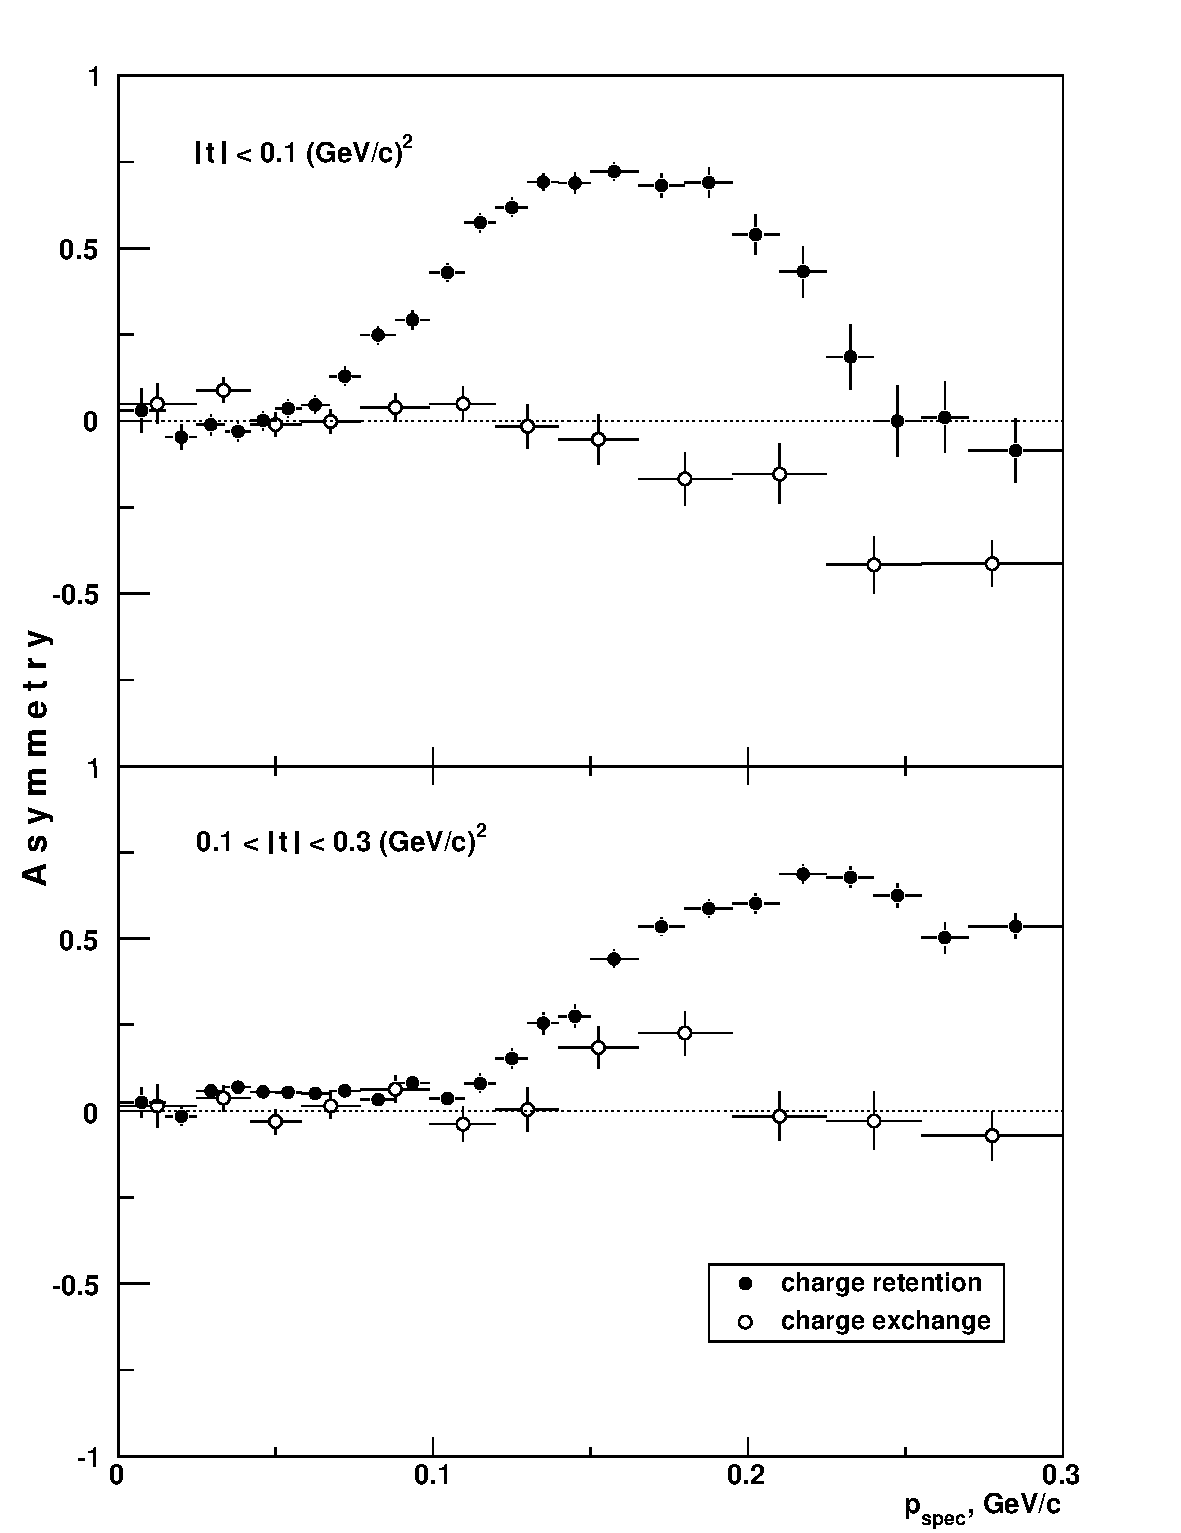
\includegraphics[width=1.00\textwidth]{asymmetry_alpha.pdf}
  \caption{Зависимость асимметрии по углу $\alpha$ от импульса спектатора
    $p_{spec}$ в системе покоя дейтрона для двух разных областей переданного
    четырёхимпульса $|t|$. Сплошные кружки~--- реакция прямого развала дейтрона
    \dpret, пустыми кружками обозначена реакция перезарядки \dpchex.}
  \label{fig:asymmetry_alpha}
\end{figure}

Таким образом, наблюдаемая сильная импульсная зависимость параметра асимметрии
по углу $\alpha$ в реакции прямого развала дейтрона вызвана взаимодействием в
конечном состоянии между протоном и нейтроном. Такое поведение может приводить
к объединению (слипанию) протона и нейтрона в конечном состоянии в дейтрон с
переходом части событий из реакции прямого развала \dpret в конкурирующий канал
реакции упругого рассеяния \dpela.

Однако, в области малых переданных импульсов $|t| < 0.1$ ГэВ/с$^2$ и импульсов
спектаторов меньших приблизительно 0.1~ГэВ/с, асимметрии по углу $\alpha$,
вызванные ВКС, практически отсутствуют (близки к нулю). Это хорошо видно
(рис.~\ref{fig:asymmetry_alpha}), как для прямого развала дейтрона, так и для
развала дейтрона с перезарядкой, где асимметрия менее выразительна и становится
отличной от нуля при заметно больших значениях импульса спектатора. Такое
поведение асимметрии по углу $\alpha$ также указывает на возможность применения
импульсного приближения в интересующей нас области малых переданных импульсов и
малых импульсов спектаторов.

Кроме вышесказанного, условие импульсного приближения означает необходимость
работать в области малых импульсов нуклонов в дейтроне, т.е. в области
преобладания $S$-волны в волновой функции дейтрона. Это видно, например из
рис.~\ref{fig:S_waves}, на котором показана вероятность $S$-волны в зависимости
от импульса внутреннего движения нуклонов в дейтроне. Согласно расчётам с
различными реалистическими потенциалами, в области до $p \simeq 0.07$~ГэВ/с
эта вероятность практически не зависит от импульса внутреннего движения нуклонов
в дейтроне и близка к единице (вне области влияния $D$-волны).

\begin{figure}[h]
  \centering
  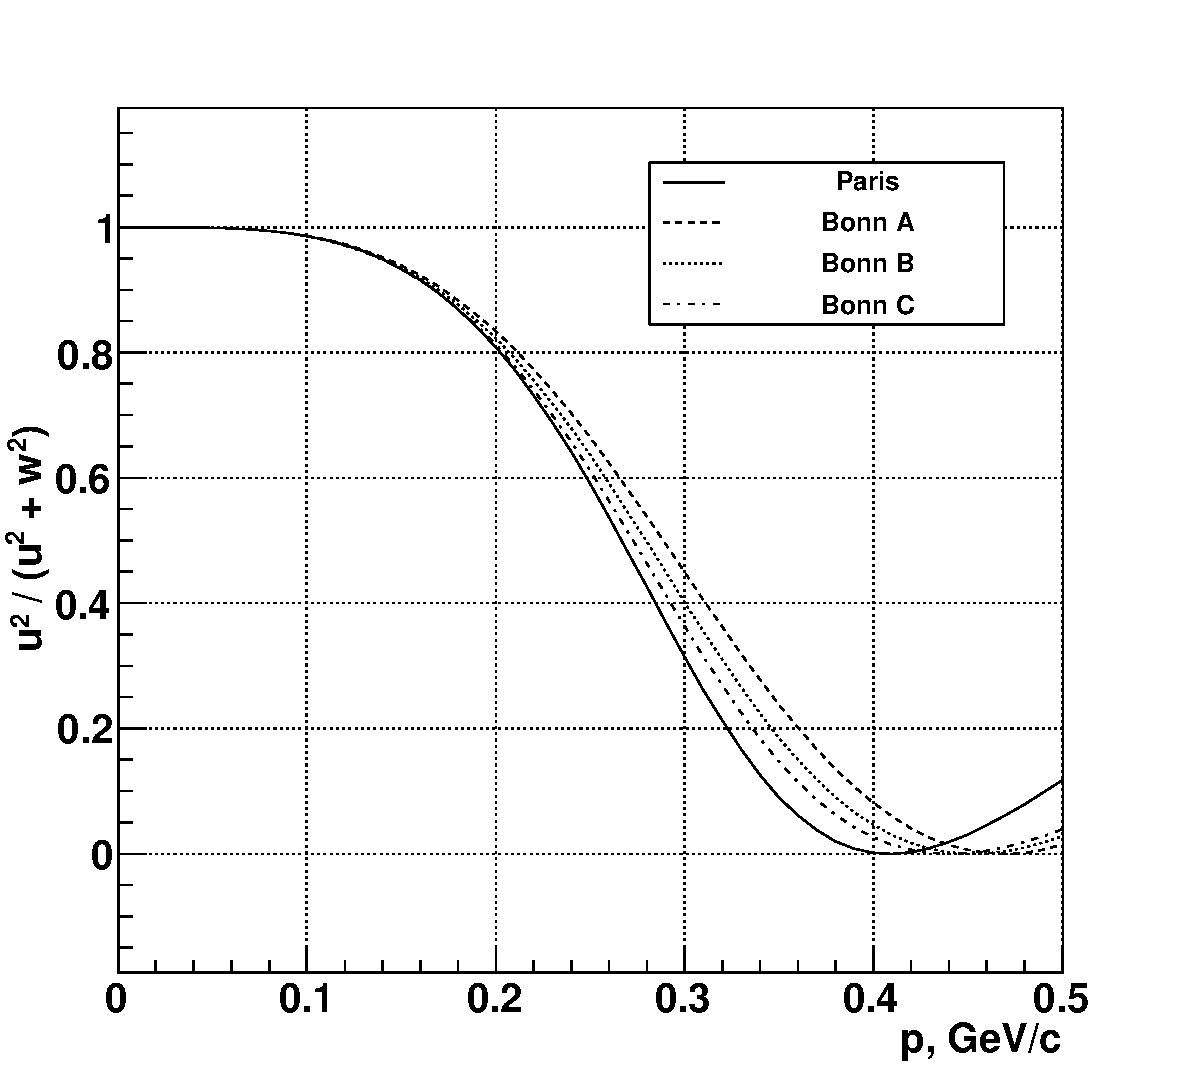
\includegraphics[width=0.79\textwidth]{S_waves.pdf}
  \caption{Вероятность $S$-волны в волновой функции дейтрона в зависимости от
    Ферми импульса $p$ нуклонов в дейтроне. $u$ и $w$~--- соответственно $S$ и
    $D$ волновые функции рассчитанные с различными реалистическими
    потенциалами.}
  \label{fig:S_waves}
\end{figure}

Предположения, при которых были выведены формулы~\eqref{eq:dpnp} и
\eqref{eq:dpnp0}, можно одновременно удовлетворить, отбирая на эксперименте
такие события, в которых в лабораторной системе координат (быстрый дейтрон
падает на покоящуюся протонную мишень) два быстрых протона из реакции
перезарядки \dpchex вылетают под малыми углами по отношению к падающему дейтрону
и с импульсами близкими к половине импульса дейтрона. Подчеркнём здесь, что
поставленная задача может быть экспериментально выполнена только при наличии
ускоренных дейтронов. В случае падающего быстрого протона на покоящуюся
дейтронную мишень, вторичные протоны из такой реакции перезарядки
$pd \rightarrow n(pp)$ будут слишком медленными, чтобы их зарегистрировать, а
сама реакция не может быть идентифицирована.

\begin{figure}[hp]
  \centering
  % 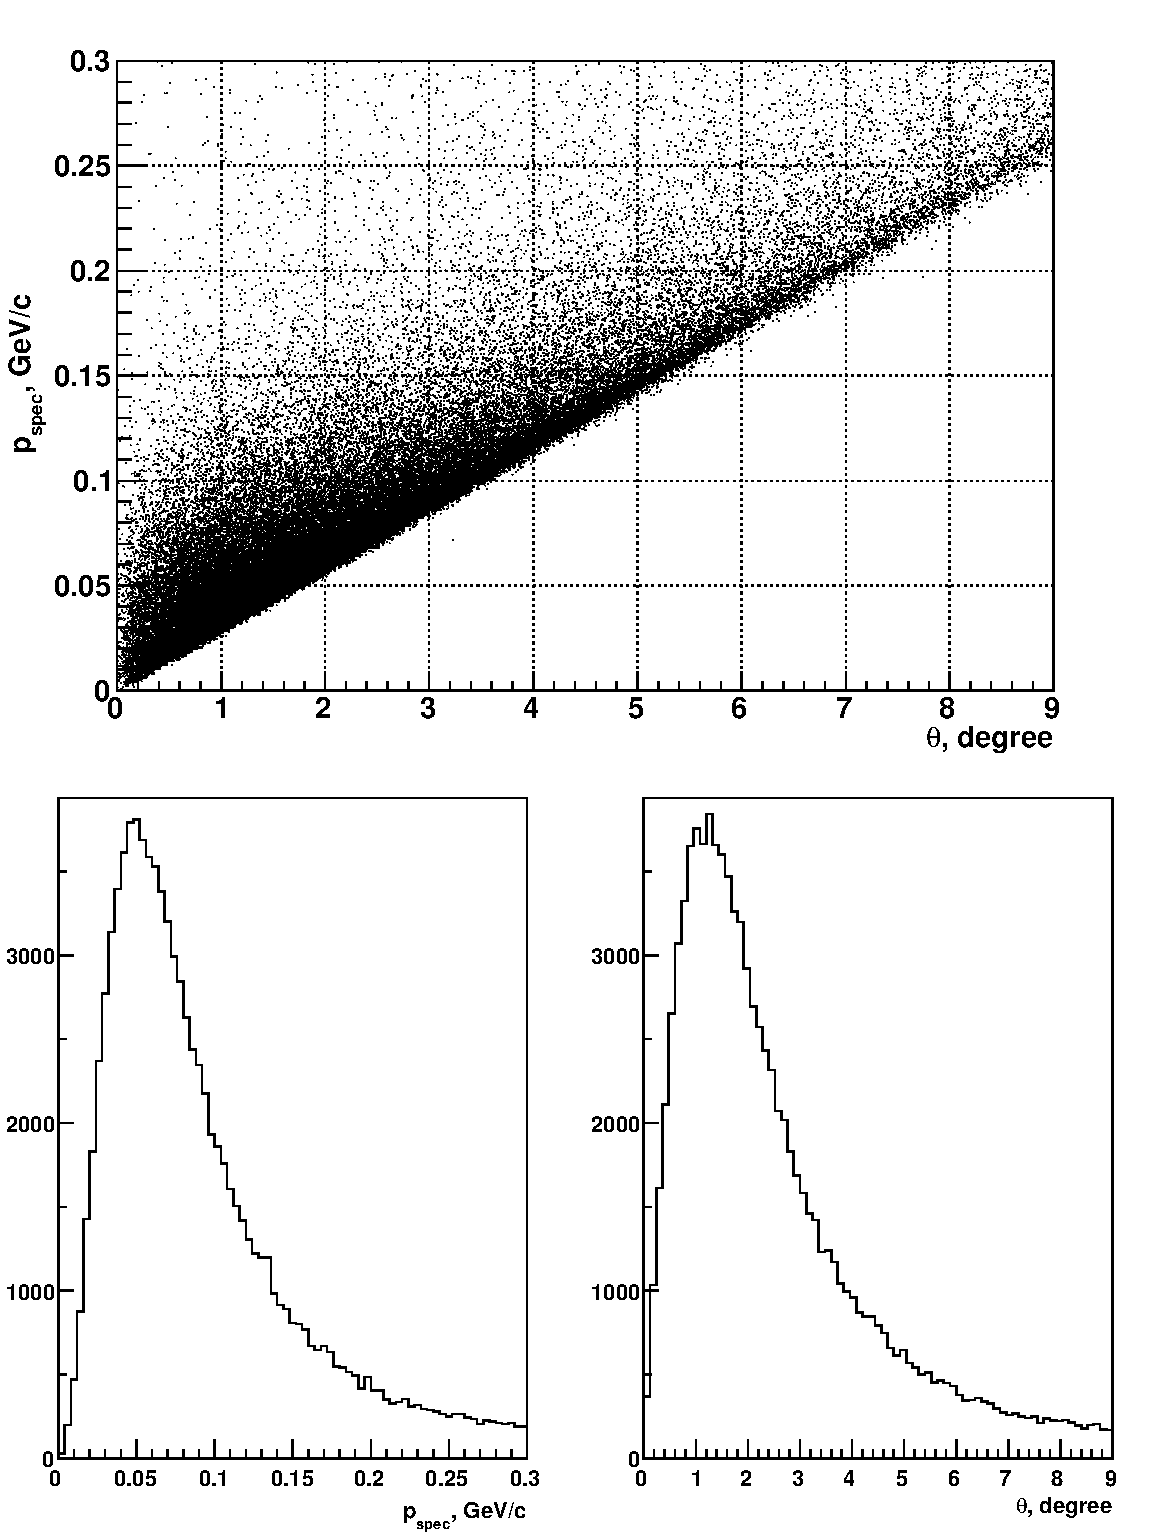
\includegraphics[width=1.00\textwidth]{theta_p.pdf}
  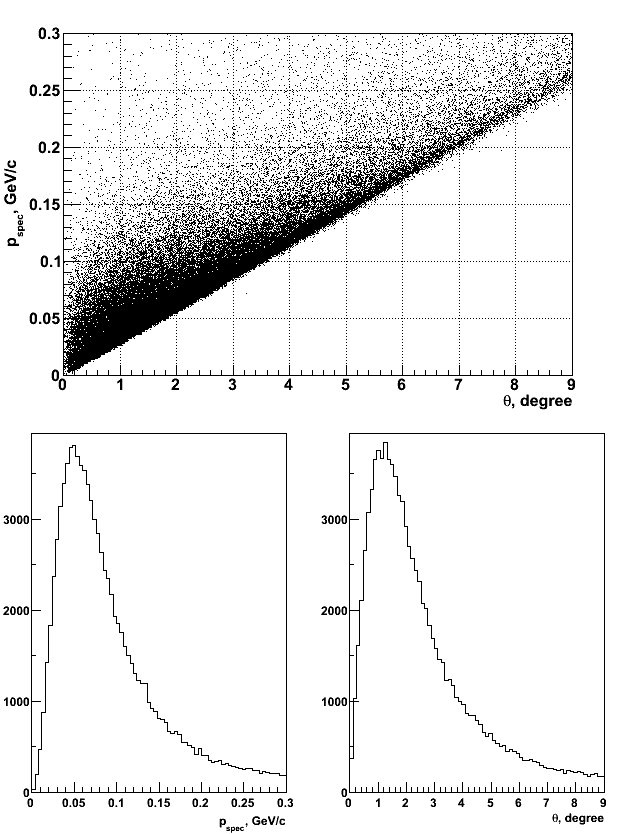
\includegraphics[width=1.00\textwidth]{theta_p.png}
  \caption{Зависимость полярного угла вылета $\theta$ спектатора в лабораторной
    системе координат от его импульса $p_{spec}$ в системе покоя дейтрона из
    реакции развала дейтрона на протоне. Под двумерным распределением показаны
    проекции на оси координат.}
  \label{fig:theta_p}
\end{figure}

Воспользуемся кинематической корреляцией между полярным углом вылета нуклона
спектатора в лабораторной системе координат и его импульсом в системе покоя
дейтрона приведённой на рис.~\ref{fig:theta_p}. Видно, что при углах меньших
порядка 5$^{\,\circ}$, или при импульсе спектатора меньше $\sim$~0.15 ГэВ/с,
лежит основная часть событий, соответствующих квази-нуклонному рассеянию. В
случае, когда передача четырёхмерного импульса (от протона-мишени к нейтрону)
стремится к нулю $|t| \rightarrow 0$, два быстрых протона из реакции перезарядки
в лабораторной системе координат имеют практически одинаковые импульсы близкие к
половине импульса дейтрона $p_{p_1} \simeq p_{p_2} \simeq (1/2)\,p_d$.

\begin{figure}[h]
  \centering
  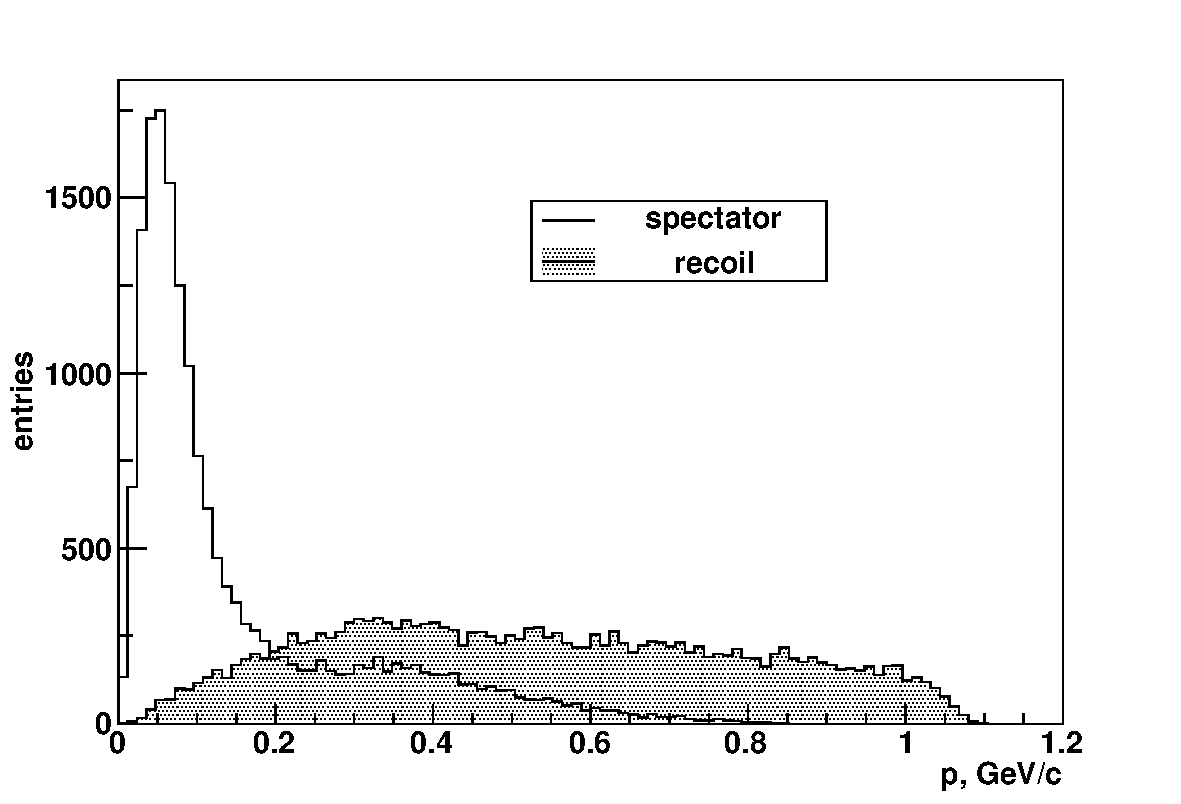
\includegraphics[width=1.00\textwidth]{spec_reco_p.pdf}
  \caption{Импульсные распределения протонов спектаторов (незаштрихованное) и
    протонов отдачи (заштрихованное) в система покоя дейтрона из реакции
    перезарядки дейтрона на протоне \dpchex.}
  \label{fig:spec_reco_p}
\end{figure}

\begin{figure}[hp]
  \centering
  \vspace{-0.2cm}
  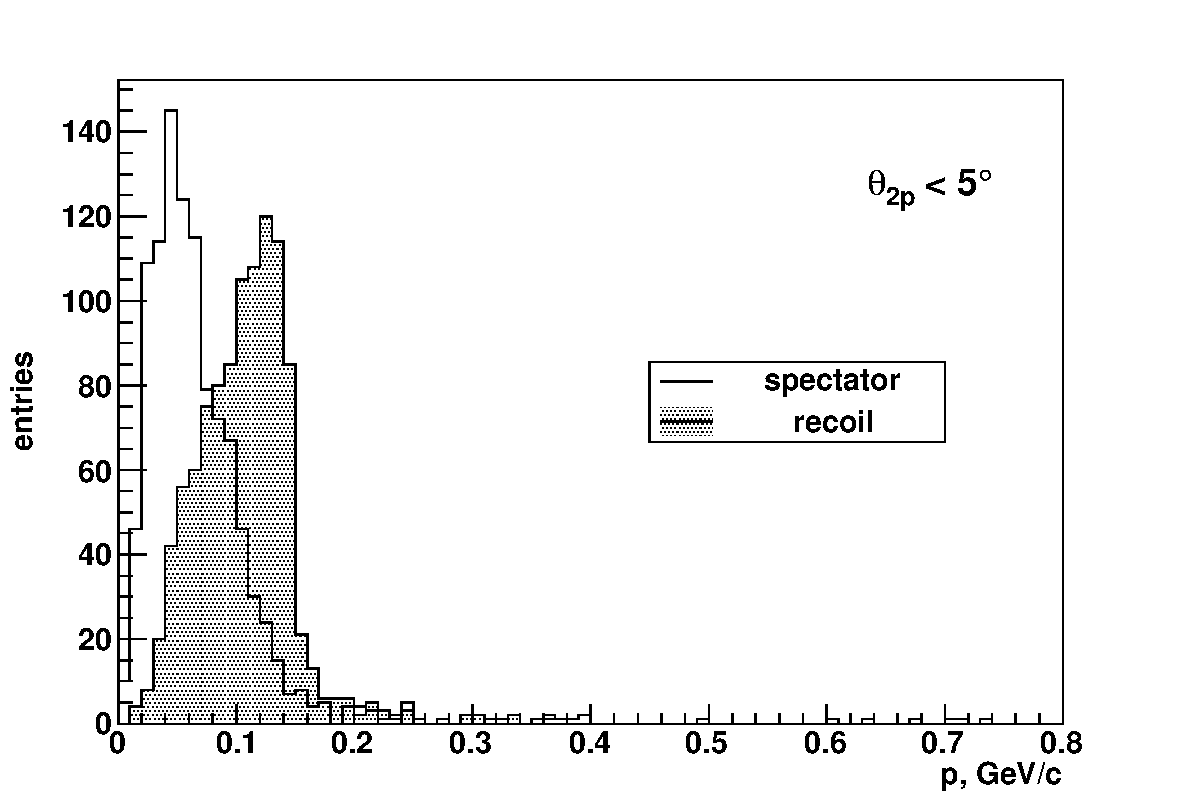
\includegraphics[width=0.99\textwidth]{spec_reco_p_5.pdf}
  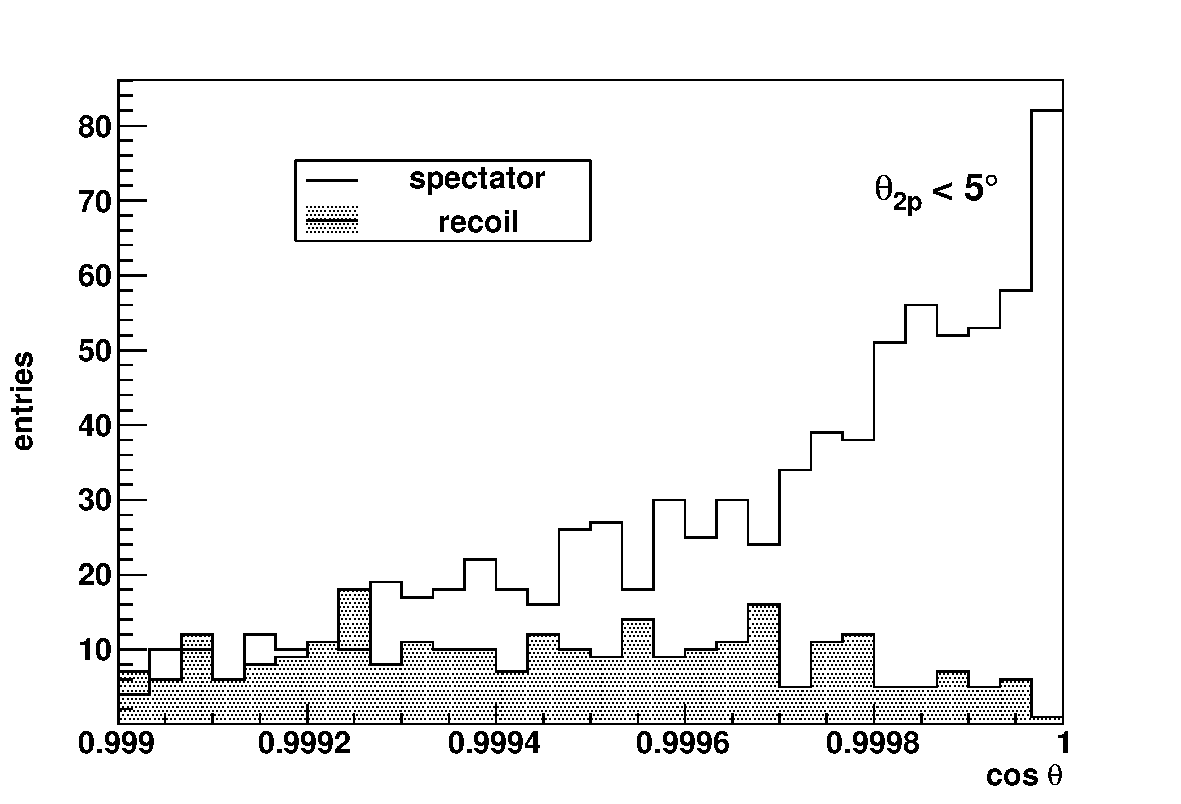
\includegraphics[width=0.99\textwidth]{spec_reco_cost_5.pdf}
  \caption{На верхнем рисунке те же самые распределения как на
    рис.~\ref{fig:spec_reco_p}, но при ограничении угла раствора конуса
    для обоих протонов в лабораторной системе координат меньше 5$^{\,\circ}$.
    Нижний рисунок~--- угловые распределения таких протонов в лабораторной
    системе координат.}
  \label{fig:spec_reco_5}
\end{figure}

Импульсные распределения двух протонов (протонов спектаторов и протонов отдачи)
из реакции перезарядки \dpchex показаны на рис.~\ref{fig:spec_reco_p}. Как
видно, если не вводить никаких ограничений на их углы вылета, импульсные
распределения этих двух протонов существенно различаются. Вид распределения
импульсов протонов спектаторов (незаштрихованное) является характерным для Ферми
движения нуклонов в дейтроне. При ограничении угла раствора конуса, в пределах
которого вылетают оба протона, в лабораторной системе координат примерно
в~5$^{\,\circ}$, распределения спектаторов и протонов отдачи значительно
перекрываются, рис.~\ref{fig:spec_reco_5}. На том же рисунке (внизу) показаны и
их угловые распределения. В итоге, отбирая события, когда пара протонов попадает
в конус с раствором меньше 5$^{\,\circ}$, будет построено распределение
дифференциального поперечного сечения реакции перезарядки дейтрона на протоне
$(d\sigma/dt)_{\dpchex}$ при малых переданных импульсах.

\subsection{События с участием промежуточной
  $\maybebm{\Delta}$-изобары.}
Прежде чем перейти к извлечению информации о вкладе спин-зависящей части
амплитуды элементарного $np$-рассеяния, необходимо оценить вклад событий с
образованием промежуточной $\Delta$-изобары. В
работах~\cite{alad75_2,alad76,alad79}
по изучению реакции безмезонного развала дейтрона на протонах было впервые
показано, что высокоимпульсная часть спектра нуклонов спектаторов в реакции
перезарядки заметно больше, чем в прямом канале. Такой эффект объяснялся вкладом
неупругих процессов с обменом промежуточной $\Delta$-изобарой, основная часть
которых является следствием квази-$pp$ столкновений, идущих через рождение
$\Delta^{++}$-изобары, диаграмма б) Фейнмана из рис.~\ref{fig:feynman}. Это
связано с большим сечением образования промежуточной $\Delta^{++}$-изобары
(канал развала дейтрона с зарядовым обменом) относительно остальных $\Delta^{+}$
и $\Delta^{\circ}$-состояний~\cite{dol86}.
% mf '\mode:=localfont; input ppn_fmf'
% mpost '\mode:=localfont; input ppn_fmf'
\begin{figure}[!h]
  \begin{center}
    \begin{fmffile}{ppn_fmf}
      \vspace{15mm}
      \hspace{-10mm}
      % pp1, delta+
      \parbox{0.45\textwidth} {
        \begin{fmfgraph*}(70,35)
          \fmfset{arrow_len}{5mm}\fmfset{arrow_ang}{10}
          \fmfleft{iA,iB}
          \fmfright{o1,o2,o3}
          \fmflabel{$d$}{iA}
          \fmflabel{$p$}{iB}
          \fmflabel{$p$}{o3}
          \fmflabel{$n$}{o2}
          \fmflabel{$p$}{o1}

          \fmf{fermion,tension=1.0}{iA,v1} % default tension=1.0
          \fmf{fermion,tension=1.0}{v2,o1}
          \fmf{fermion,tension=1.0}{v2,o2}
          \fmf{fermion,tension=1.0}{iB,v3,o3}

          \fmf{fermion,tension=1.5,label=$n$}{v1,v2}
          \fmf{fermion,tension=0.2,lab.side=left,label=$p$}{v1,v3}
          \fmf{fermion,tension=0.1,lab.side=left,label=$\Delta^{+}$}{v3,v2}

          \fmfblob{0.06w}{v1}
          \fmfdot{v2,v3}
          \fmf{dbl_plain_arrow}{iA,v1}
          \fmffreeze
          \fmf{plain_arrow,width=2.5*thin}{v3,v2}
        \end{fmfgraph*}
      }
      % pp2, delta++
      \qquad
      \parbox{0.45\textwidth} {
        \begin{fmfgraph*}(70,35)
          \fmfset{arrow_len}{5mm}\fmfset{arrow_ang}{10}
          \fmfleft{iA,iB}
          \fmfright{o1,o2,o3}
          \fmflabel{$d$}{iA}
          \fmflabel{$p$}{iB}
          \fmflabel{$n$}{o3}
          \fmflabel{$p$}{o2}
          \fmflabel{$p$}{o1}

          \fmf{fermion,tension=1.0}{iA,v1} % default tension=1.0
          \fmf{fermion,tension=1.0}{v2,o1}
          \fmf{fermion,tension=1.0}{v2,o2}
          \fmf{fermion,tension=1.0}{iB,v3,o3}

          \fmf{fermion,tension=1.5,label=$n$}{v1,v2}
          \fmf{fermion,tension=0.2,lab.side=left,label=$p$}{v1,v3}
          \fmf{fermion,tension=0.1,lab.side=left,label=$\Delta^{++}$}{v3,v2}

          \fmfblob{0.06w}{v1}
          \fmfdot{v2,v3}
          \fmf{dbl_plain_arrow}{iA,v1}
          \fmffreeze
          \fmf{plain_arrow,width=2.5*thin}{v3,v2}
        \end{fmfgraph*}
      }
      \begin{center}
        \vspace{5mm}
        а) \hspace{75mm} б)
      \end{center}
      % np1, delta+
      \vspace{15mm}
      \hspace{-10mm}
      \parbox{0.45\textwidth} {
        \begin{fmfgraph*}(70,35)
          \fmfset{arrow_len}{5mm}\fmfset{arrow_ang}{10}
          \fmfleft{iA,iB}
          \fmfright{o1,o2,o3}
          \fmflabel{$d$}{iA}
          \fmflabel{$p$}{iB}
          \fmflabel{$n$}{o3}
          \fmflabel{$p$}{o2}
          \fmflabel{$p$}{o1}

          \fmf{fermion,tension=1.0}{iA,v1} % default tension=1.0
          \fmf{fermion,tension=1.0}{v2,o1}
          \fmf{fermion,tension=1.0}{v2,o2}
          \fmf{fermion,tension=1.0}{iB,v3,o3}

          \fmf{fermion,tension=1.5,label=$p$}{v1,v2}
          \fmf{fermion,tension=0.2,lab.side=left,label=$n$}{v1,v3}
          \fmf{fermion,tension=0.1,lab.side=left,label=$\Delta^{+}$}{v3,v2}

          \fmfblob{0.06w}{v1}
          \fmfdot{v2,v3}
          \fmf{dbl_plain_arrow}{iA,v1}
          \fmffreeze
          \fmf{plain_arrow,width=2.5*thin}{v3,v2}
        \end{fmfgraph*}
      }
      % np2, delta0
      \qquad
      \parbox{0.45\textwidth} {
        \begin{fmfgraph*}(70,35)
          \fmfset{arrow_len}{5mm}\fmfset{arrow_ang}{10}
          \fmfleft{iA,iB}
          \fmfright{o1,o2,o3}
          \fmflabel{$d$}{iA}
          \fmflabel{$p$}{iB}
          \fmflabel{$p$}{o3}
          \fmflabel{$n$}{o2}
          \fmflabel{$p$}{o1}

          \fmf{fermion,tension=1.0}{iA,v1} % default tension=1.0
          \fmf{fermion,tension=1.0}{v2,o1}
          \fmf{fermion,tension=1.0}{v2,o2}
          \fmf{fermion,tension=1.0}{iB,v3,o3}

          \fmf{fermion,tension=1.5,label=$p$}{v1,v2}
          \fmf{fermion,tension=0.2,lab.side=left,label=$n$}{v1,v3}
          \fmf{fermion,tension=0.1,lab.side=left,label=$\Delta^{\circ}$}{v3,v2}

          \fmfblob{0.06w}{v1}
          \fmfdot{v2,v3}
          \fmf{dbl_plain_arrow}{iA,v1}
          \fmffreeze
          \fmf{plain_arrow,width=2.5*thin}{v3,v2}
        \end{fmfgraph*}
      }
      \begin{center}
        \vspace{5mm}
        в) \hspace{75mm} г)
      \end{center}
    \end{fmffile}

    \caption{Диаграммы Фейнмана для реакции безмезонного развала дейтрона на
      протоне \dpfrag с образованием промежуточной $\Delta$-изобары. Диаграммы
      а) и б) соответствуют событиям с участием $\Delta^{+}$ и
      $\Delta^{++}$-изобары в квази-$pp$ столкновениях. События с обменом заряда
      изображены на диаграммах б) и в).}
    \label{fig:feynman}
  \end{center}
\end{figure}



%%% Local Variables:
%%% mode: latex
%%% TeX-master: "../musinsky_disser"
%%% coding: utf-8
%%% End:


Импульсные распределения нуклонов спектаторов (нормированные на максимум) из
реакции перезарядки на дейтроне \dpchex и реакции прямого канала с сохранением
заряда \dpret в системе покоя дейтрона показаны на
рис.~\ref{fig:resonance_spec}. Заштрихованная область высокоимпульсной части
спектра нуклонов спектаторов, из канала перезарядки, представляет относительный
избыток событий, который связан с долей промежуточных изобарных состояний. В
связи с заметным вкладом этих событий было необходимо ввести соответствующую
поправку. Однако, из сопоставления рис.~\ref{fig:theta_p} и
рис.~\ref{fig:resonance_spec} видно, что этот избыток находится в области
импульсов выше $\sim$~0.2~ГэВ/с, т.е. вне конуса с углом раствора в
5$^{\,\circ}$, и таким образом, не влияет на дифференциальное сечение реакции
перезарядки при $|t|$ вблизи нуля.

\begin{figure}[h]
  \centering
  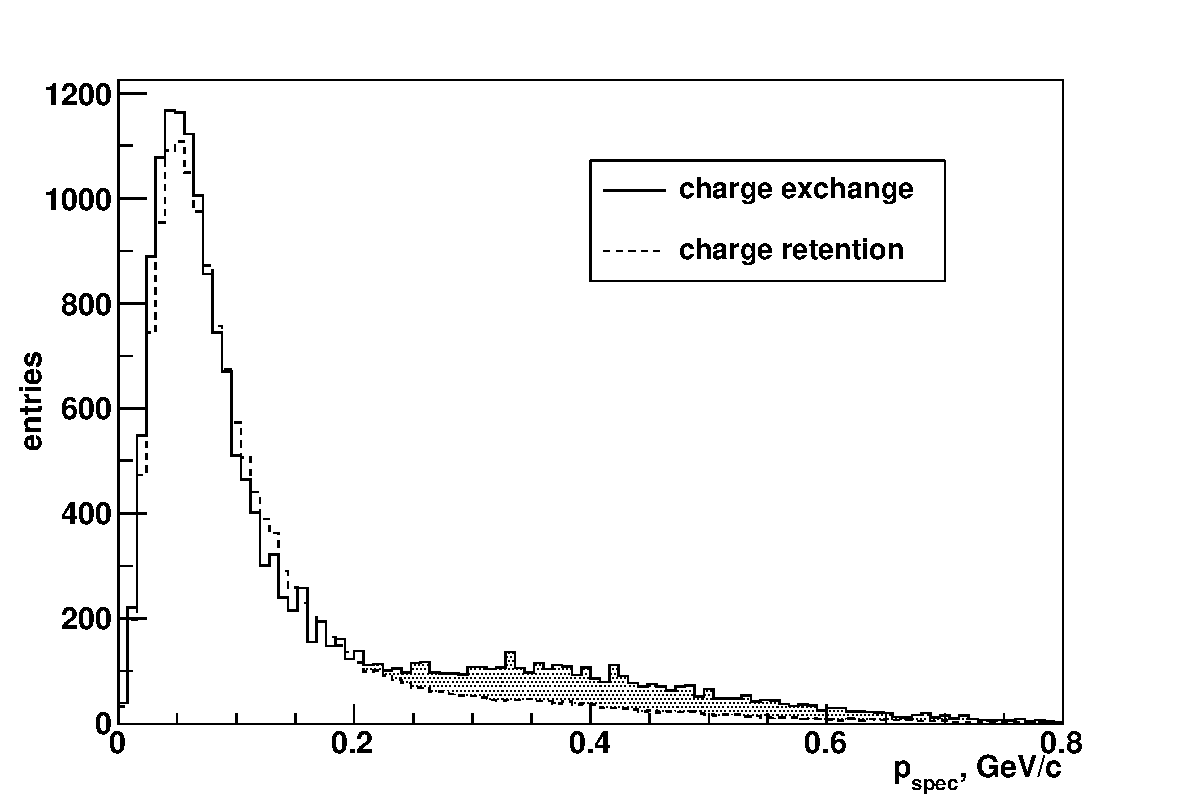
\includegraphics[width=1.00\textwidth]{resonance_spec.pdf}
  \caption{Импульсные распределения нуклонов спектаторов из реакции прямого
    канала (штриховая линия) и перезарядки (сплошная) нормированные на максимум.
    Заштрихованная область ($p_{spec} \gtrsim 0.2$~ГэВ/с) представляет избыток
    событий связанный с образованием промежуточной $\Delta$-изобары.}
  \label{fig:resonance_spec}
\end{figure}

\section{Оценка вклада спин-зависящей части амплитуды
  \maybebm{{\np}} рассеяния}
Проведённый анализ экспериментальных данных по реакции перезарядки дейтрона на
протоне-мишени, даёт возможность получить информацию о спиновой зависимости
обменного $np$-рассеяния назад. Для ответа, на интересующий нас вопрос о вкладе
спин-зависящей части амплитуды элементарного \np процесса, необходимо, как уже
говорилось раньше, кроме измерения дифференциального поперечного сечения
$(d\sigma/dt)_{\dpchex}$ в реакции \dpchex, привлечь и результаты экспериментов
по измерению дифференциального сечения $(d\sigma/dt)_{\np}$ реакции элементарной
перезарядки \np при $|t|=0$.

В разделе~\ref{section:npnp} первой главы было показано, что среди имеющихся в
литературе экспериментальных данных для $np$-рассеяния, измерения сделанные
Бизардом~и~др. на ускорителе Сатурн~\cite{biz75} являются наиболее корректными и
самыми близкими по энергии. На их основе мы получили зависимость
(выражение~\eqref{eq:np0}, стр.~\pageref{eq:np0}) дифференциального поперечного
сечения $(d\sigma/dt)_{\np}$ при $|t|=0$ от импульса нуклона в элементарной
реакции перезарядки \np. Для импульса 1.675~ГэВ/с на нуклон получаем
величину $(d\sigma/dt)_{\np}\,|\,_{t=0} = 54.7 \pm 0.2$~мб/(ГэВ/с)$^{2}$.

Определим теперь на основе наших экспериментальных данных значение
дифференциального поперечного сечения $(d\sigma/dt)_{\dpchex}$ изучаемой реакции
перезарядки на дейтроне \dpchex при $|t|=0$ и импульсе дейтрона 3.35~ГэВ/с. Для
набора пар быстрых протонов, попадающих в конус с раствором меньше
5$^{\,\circ}$, строится распределение сечения с учётом миллибарн-эквивалента
события и поправки, равной отношению полного числа спектаторных нуклонов к числу
спектаторов в выбранном конусе. Полученное распределение сечения
аппроксимируется выражением
\begin{equation}
  \label{eq:exdp}
  d\sigma/dt = p_0\exp(p_1\,t + p_2\,t^2)
\end{equation}
в интервале $t$ од 0 до 0.01 (ГэВ/с)$^2$ и приведено на
рис.~\ref{fig:dp_two_protons}. Экстраполяция к $t=0$ дала значение
$(d\sigma/dt)_{\dpchex}\,|\,_{t=0} = 30.2 \pm 4.1$~мб/(ГэВ/с)$^{2}$. Заметим,
что тем же самым способом (вид функции и интервал аппроксимации) были получены
и сечения элементарной перезарядки нейтрона на протоне.

\begin{figure}[h]
  \centering
  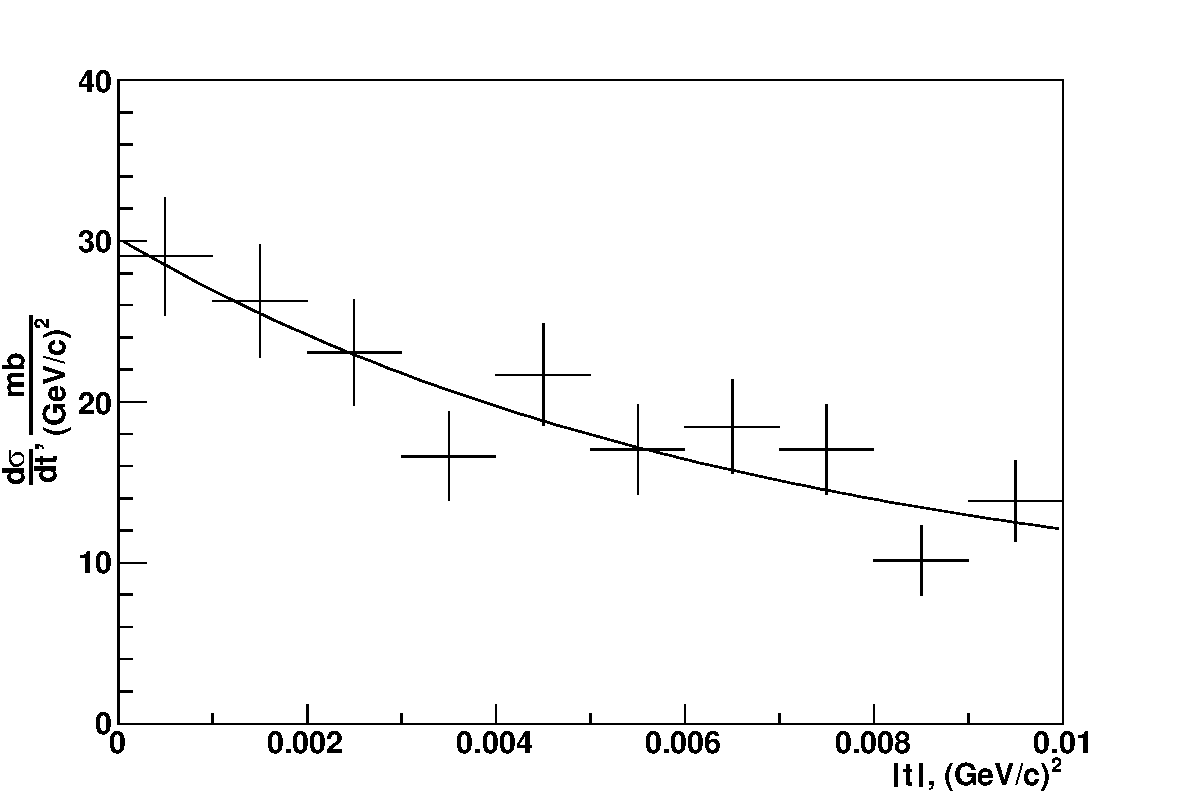
\includegraphics[width=1.00\textwidth]{dp_two_protons.pdf}
  \caption{Распределение дифференциального поперечного сечения реакции с обменом
    заряда \dpchex при малых значениях $|t|$. Сплошная линия~--- аппроксимация
    функцией \eqref{eq:exdp}.}
  \label{fig:dp_two_protons}
\end{figure}

Если бы дифференциальное поперечное сечение перезарядки на дейтроне при $|t|=0$
равнялось точно 2/3 от дифференциального сечения элементарной \np перезарядки
также при $|t|=0$, то это бы означало, согласно выше приведённой
формуле~\eqref{eq:dpnp0}, что амплитуда перезарядки была бы полностью
спин-зависящей. Однако на эксперименте такой закономерности не наблюдается.
Из-за этого было введено отношение $R$, через посредство которого удобно
извлекать долю спин-зависящей (а также и спин-независящей) части амплитуды
реакции \np перезарядки. Величина $R$ используется во многих работах по
интересующей нас теме исследований.

Введём отношение $R_{\np}$ дифференциальных сечений для реакции перезарядки на
дейтроне \dpchex и реакции элементарной перезарядки \np
\begin{equation}
  R_{\np} = \frac{(d\sigma/dt)_{\dpchex}}{(d\sigma/dt)_{\np}}\,.
\end{equation}
При нулевом переданном импульсе $|t|=0$ отношение $R_{\np}$, исходя из
формулы~\eqref{eq:dpnp0}, определяет вклад спин-зависящей части амплитуды
$np$-рассеяния назад, и его можно записать как
\begin{equation}
  R_{\np} = \frac{2}{3}\,\frac{(d\sigma/dt)^{SD}_{\np}}{(d\sigma/dt)_{\np}}\,.
\end{equation}
Из измеренного нами сечения $(d\sigma/dt)_{\dpchex}\,|\,_{t=0} = 30.2 \pm
4.1$~мб/(ГэВ/с)$^{2}$ и сечения $(d\sigma/dt)_{\np}\,|\,_{t=0} = 54.7 \pm
0.2$~мб/(ГэВ/с)$^{2}$ определённого на основе данных Бизардa~и~др. получаем
значение
\begin{equation}
  R_{\np} = 0.55 \pm 0.08\,,
\end{equation}
означающее преобладающий вклад спин-зависящей части амплитуды реакции
перезарядки нейтрона на протоне~\cite{gla_mucha08}.

Исходя из формул~\eqref{eq:np} и \eqref{eq:dpnp0}, отношение $R_{\np}$ может
быть приравнено к
\begin{equation}
  R_{\np} = \frac{2/3\,(d\sigma/dt)^{SD}_{\np}}
  {(d\sigma/dt)^{SI}_{\np} + (d\sigma/dt)^{SD}_{\np}}
\end{equation}
и, соответственно, доля спин-независящей части сечения $R^{\,ID}_{\np}$ реакции
упругой \np перезарядки равна
\begin{equation}
  R^{\,ID}_{\np} = \frac{(d\sigma/dt)^{SI}_{\np}}{(d\sigma/dt)^{SD}_{\np}} =
  \frac{2}{3\,R_{\np}} \ - \ 1 = 0.21 \pm 0.17\,.
\end{equation}

На рис.~\ref{fig:R_np} показана зависимость величины $R_{\np}$ от кинетической
энергии нейтрона в лабораторной системе координат в сравнении с результатами
других экспериментов. Видно, что полученное нами значение находится в согласии,
как с более ранними~\cite{pag88,lehar09}, так и с недавно опубликованными
результатами группы Дельта-Сигма~\cite{shar09} при более высоких энергиях.

\begin{figure}[!h]
  \centering
  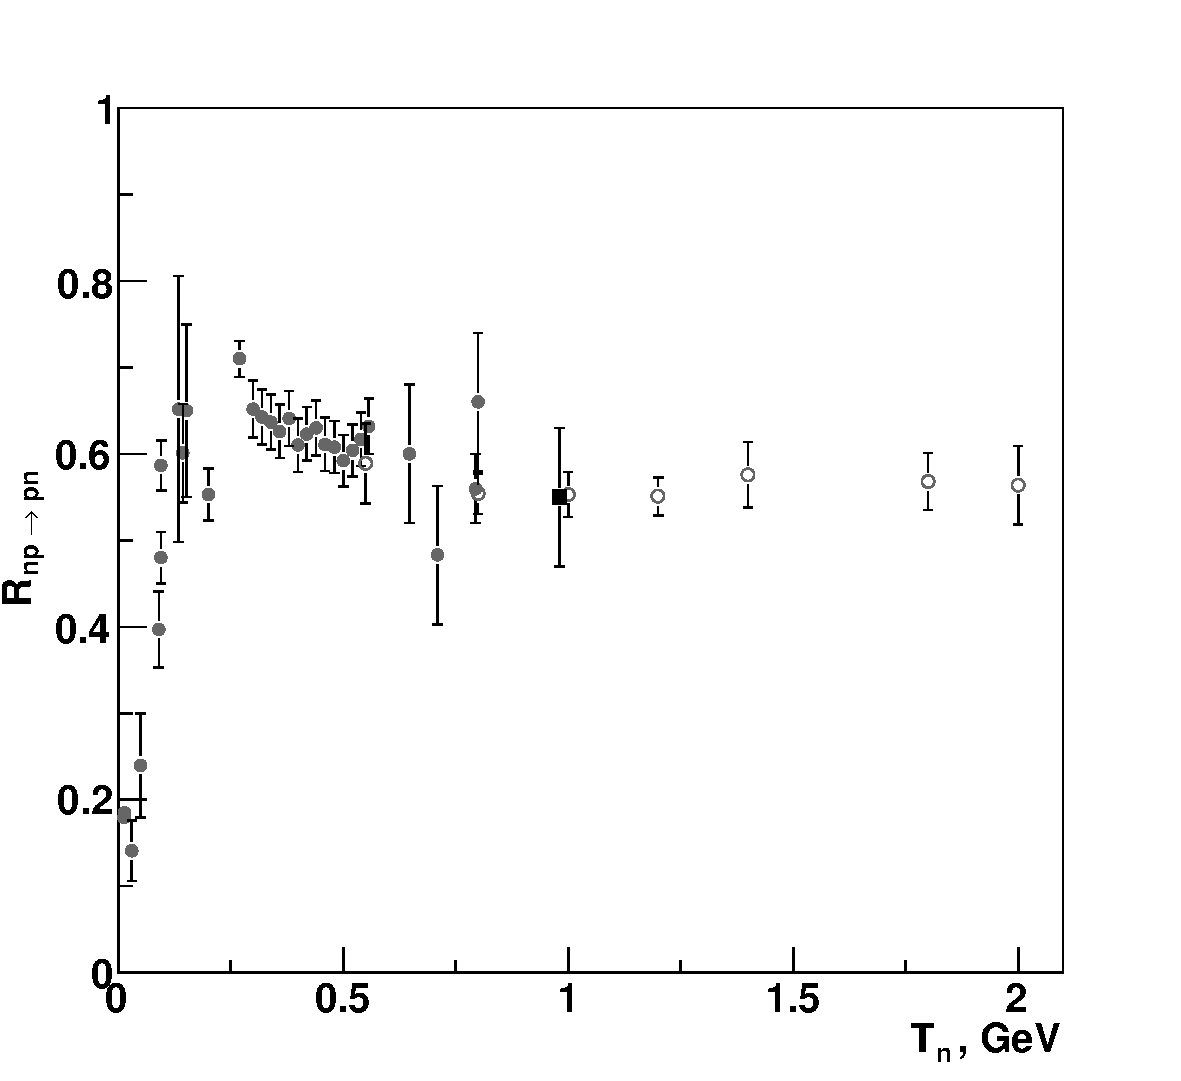
\includegraphics[width=1.00\textwidth]{R_np.pdf}
  \caption{Зависимость величины $R_{\np}$ от кинетической энергии нейтрона
    $T_n$. Сплошные кружки представляют значения полученные в более ранних
    экспериментах, квадратик ($T_n = 0.98$~ГэВ)~--- определённое нами значение
    величины $R_{\np}$, пустые кружки~--- недавно опубликованные результаты
    эксперимента Дельта-Сигма~\cite{shar09}.}
  \label{fig:R_np}
\end{figure}

В работе~\cite{alad75_2} была осуществлена попытка получить экспериментальную
оценку вклада спин-зависящей части амплитуды элементарного \np процесса,
основанную на описании дифференциального поперечного сечения реакции \dpchex,
полученного с помощью водородной камеры через известные к тому времени
экспериментальные данные по $np$-рассеянию. Однако, статистика событий реакции
перезарядки на дейтрона была невелика и данные по $np$-рассеянию были
неоднозначны. Соответственно, и полученная оценка вклада была также
неоднозначна, хотя и указывала на значительную роль зависящей от спина части в
амплитуде \np перезарядки.

В пучке дейтронов это была первая и единственная работа. Следует отметить, что
все более ранние работы на эту тему были проведены в квази-нейтронных вторичных
пучках, получавшихся коллимированными вторичными нейтронами довольно широкого
импульсного спектра. Позже, на эксперименте Дельта-Сигма~\cite{shar09}, где
использовались квази-монохроматические нейтроны от стриппинга выведенных из
ускорителя монохроматических дейтронов, удалось существенно сузить спектр
такого нейтронного пучка.

\section{Выводы ко второй главе}
В итоге выполнения экспериментальной программы, описанной в настоящей главе,
были получены следующие результаты:
\begin{list}{\labelitemi}{\leftmargin=1em}
\item Проведён полный анализ $dp$-взаимодействий, полученных с помощью 100-см
  водородной пузырьковой камеры ЛВЭ ОИЯИ облучённой в пучке дейтронов при
  импульсе 3.35~ГэВ/с.
\item Получены значения сечений 17 каналов $dp$-взаимодействий и оценены потери
  событий. Качество полученной экспериментальной информации свидетельствовало о
  её пригодности для последующего физического анализа.
\item Определено значение миллибарн эквивалента, необходимого для определения
  дифференциального сечения $d\sigma/dt$ реакции с обменом заряда \dpchex при
  $t = 0$.
\item Исследована реакция перезарядки дейтрона на протоне в эксклюзивной
  постановке c целью определения вклада спин-зависящей амплитуды \np перезарядки
  на основе прямого измерения дифференциального сечения $d\sigma/dt$ при $t = 0$
  и обоснована применимость использованного нами подхода. Определено
  дифференциальное сечение реакции перезарядки
  $(d\sigma/dt)_{\dpchex}\,|\,_{t=0} = 30.2 \pm 4.1$~мб/(ГэВ/с)$^{2}$.
\item Впервые в пучке дейтронов получено отношение $R_{\np}$ дифференциальных
  сечений перезарядки при $t=0$ в реакции \dpchex и \np и в рамках импульсного
  приближения получено
  значение $R_{\np} = 0.55\,\pm\,0.08$, что свидетельствует о преобладающем
  вкладе спин-зависящей части амплитуды \np рассеяния и согласуется с данными
  других экспериментов в области близких энергий.
\end{list}

%%% Local Variables:
%%% mode: latex
%%% TeX-master: "musinsky_disser"
%%% coding: utf-8
%%% End:
